\section{Minimizing the size of the transmitted messages}
\todo{I proposed a new text for this part, it is in green}
To minimize the forwarded data size, first of all we have to get rid of the names of each data. To keep the data readable for the receiver, we can either use a character to separate each segment of data, or we can agree upon a constant size for each segment of data.

The former code encoded each digit of a decimal number as an ASCII character. It means that the number segment only used 10 out of the 256 possible characters. To compress data, we should utilize all the ASCII characters. One way to do it is to make a character store the number as its address in the 8 bit address table. We basically have to convert the numbers to base 256.

We utilized Labview's \todo{maybe we should move it to implementation} built in flatten to string node, which basically converts numeric data to the correspondent string. For example, it convert an 8 bit integer to the correspondent ASCII character. If the sbRIO and the PC uses the same encoding, they can basically send bitcode as if it was string then decode it by doing a simple conversion.
 
\todo{please specify formally the new and old protocol}

For each arm, the sbRIO must send encoder, potmeter and current measurement data from each of the seven motors. Each data is represented as a 32 bit float. This adds up to 48 bytes of data to be sent each cycle. The described method sends 48 byte long strings not including the header. The former method sends 67 characters for formatting and naming purposes and 96 bytes of numeric data, assuming each double number is sent in 8 digits. It adds up to 163 bytes.

By removing the names from the string and compressing a data, the string can become 70 percents shorter, which is a valuable increase in efficiency.

%%%%%%%%%%%%%%%%%%%%%%%%%%%%%%%%%%%%%%%%%%%%%%%%%%%%%%%%%%%%
\textcolor{\color{green}}{
There are two elements that impact greatly the size of the exchanged messages: the number of character added by the JSON format and the length of the numbers.
As detailed in ~\subsecref{subsec:JSON}, the JSON format add numerous characters for the structure and require a name for each value. The first modification made in order to minimize the size of the messages was to remove the JSON format. To do so it is necessary to agree upon a fixed format for the messages. For simplicity, it was decided to keep a format similar to the original one, composed of a vector of positions, a vector of velocities and a vector of efforts. All of these vectors contain the same number of elements and each elements must have the same length to make it possible to read. In addition to these three vectors, a vector of booleans was added in order to keep the possibility of enabling or disabling the motors.}

\textcolor{\color{green}}{As mentioned, all the numbers in the vectors should have the same length. In the original format, not only the numbers were long (18 digits) but the length would vary from one message to another. Different solutions were considered. The first one would be to fix the number of digits but that would still imply a conversion to string. The second solution considered was the compression of the characters sent. However, as the size of the messages is small the compression rate is low (20\% at best\todo{ref}) the computation time required for compression would end up in a low gain of time or even in a time loss. The third and last option was to send the bitcode directly without any encoding. The numerical values being stored as floats each of them requires 4 bytes and that also have the advantage of having a fixed length without having to round the value. The last solution was chosen as it is the one with which the message sent is the shortest with the lowest computation time as there is no encoding of any kind. The only issue is that the endianness of both devices is not the same, this is fixed in the implementation on the ROS side. The packets obtained with the new format are shown in \figref{fig:received_packet} and \figref{fig:sent_packet}

}
%%%%%%%%%%%%%%%%%%%%%%%%%%%%%%%%%%%%%%%%%%%%%%%%%%%%%%%%%%%%

\begin{figure}[H]
\centering
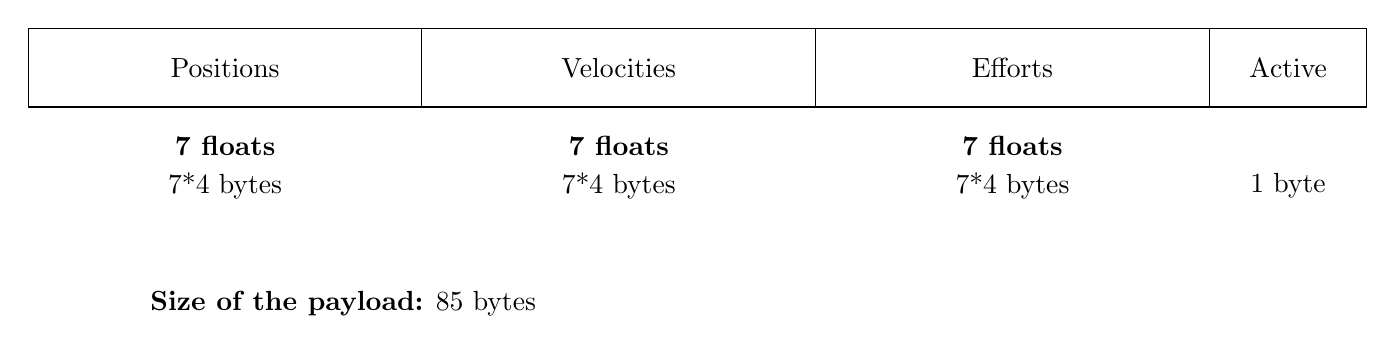
\begin{tikzpicture}

\draw (0,0) rectangle (17,1);
\draw (0,0) rectangle (5,1);
\draw (0,0) rectangle (10,1);
\draw (0,0) rectangle (15,1);

\node at (2.5,0.5) {Positions};
\node at (7.5,0.5) {Velocities};
\node at (12.5,0.5) {Efforts};
\node at (16,0.5) {Active};

\node at (2.5,-0.5) {\textbf{7 floats}};
\node at (7.5,-0.5) {\textbf{7 floats}};
\node at (12.5,-0.5) {\textbf{7 floats}};
%\node at (16,-0.5) {\textbf{n booleans}};

\node at (2.5,-1) {7*4 bytes};
\node at (7.5,-1) {7*4 bytes};
\node at (12.5,-1) {7*4 bytes};
\node at (16,-1) {1 byte};

\node at (4,-2.5) {\textbf{Size of the payload:} 85 bytes}; %I have no idea why i need to put 4 as a coordinate for it to not mess up the rest of the figure
\end{tikzpicture}
\caption{Packet from the sbRIO to ROS for one arm}
\label{fig:received_packet}
\end{figure}

\begin{figure}[H]
\centering
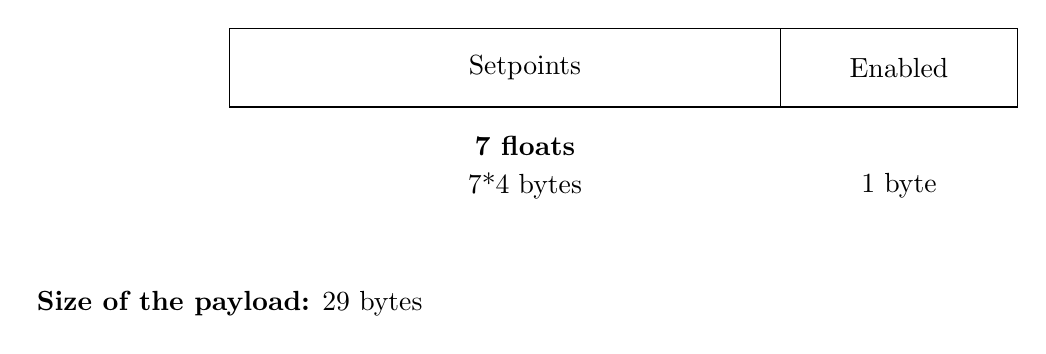
\begin{tikzpicture}

\draw (0,0) rectangle (10,1);
\draw (0,0) rectangle (7,1);

\node at (3.75,0.5) {Setpoints};
\node at (8.5,0.5) {Enabled};

\node at (3.75,-0.5) {\textbf{7 floats}};
%\node at (8.5,-0.5) {\textbf{n booleans}};

\node at (3.75,-1) {7*4 bytes};
\node at (8.5,-1) {1 byte};

\node at (0,-2.5) {\textbf{Size of the payload:} 29 bytes}; 
\end{tikzpicture}
\caption{Packet from ROS to the sbRIO for one arm}
\label{fig:sent_packet}
\end{figure}